\documentclass[letter]{article}
\usepackage{amsmath}
\usepackage{amsfonts}
\usepackage{amssymb}
\usepackage{ifthen}
\usepackage{fancyhdr}
\usepackage{graphicx}
\usepackage{subcaption}
\usepackage[shortlabels]{enumitem}

%%%
% Set up the margins to use a fairly large area of the page
%%%
\oddsidemargin=.2in
\evensidemargin=.2in
\textwidth=6in
\topmargin=0in
\textheight=9.0in
\parskip=.07in
\parindent=0in
\pagestyle{fancy}

%%%
% Set up the header
%%%
\newcommand{\setheader}[6]{
	\lhead{{\sc #1} {\sc #2}\\{} ({\small \it \today})}
	\rhead{
		{\bf #3} 
		\ifthenelse{\equal{#4}{}}{}{(#4)}\\
		{\bf #5} 
		\ifthenelse{\equal{#6}{}}{}{(#6)}%
	}
}

\begin{document}
	\setheader{CSC490}{Module 1}{Qiwen Hua}{}{Ben Weisz}{}
	
	\setcounter{section}{2}
	\subsection{LiDAR Voxelization}

	\textbf{Part 2:} In the implementation of the \verb|Voxelizer.forward| function, we map raw LiDAR points to voxels by taking the difference between the points and bounds (e.g. \verb|x_max|) and scale down by `step`. Therefore, larger \verb|step| yields lower resolution for the voxelized point clouds, thus decreases the amount of captured information. 

	We can visualize the conclusion above by plotting the voxelized LiDAR point clouds for scene \verb|000| with four different \verb|step|s $\in \{0.25, 0.50, 1.00, 2.00\}$. The plots are shown below:

	\begin{figure}[h]
		\begin{subfigure}[t]{\textwidth}
			\centering
			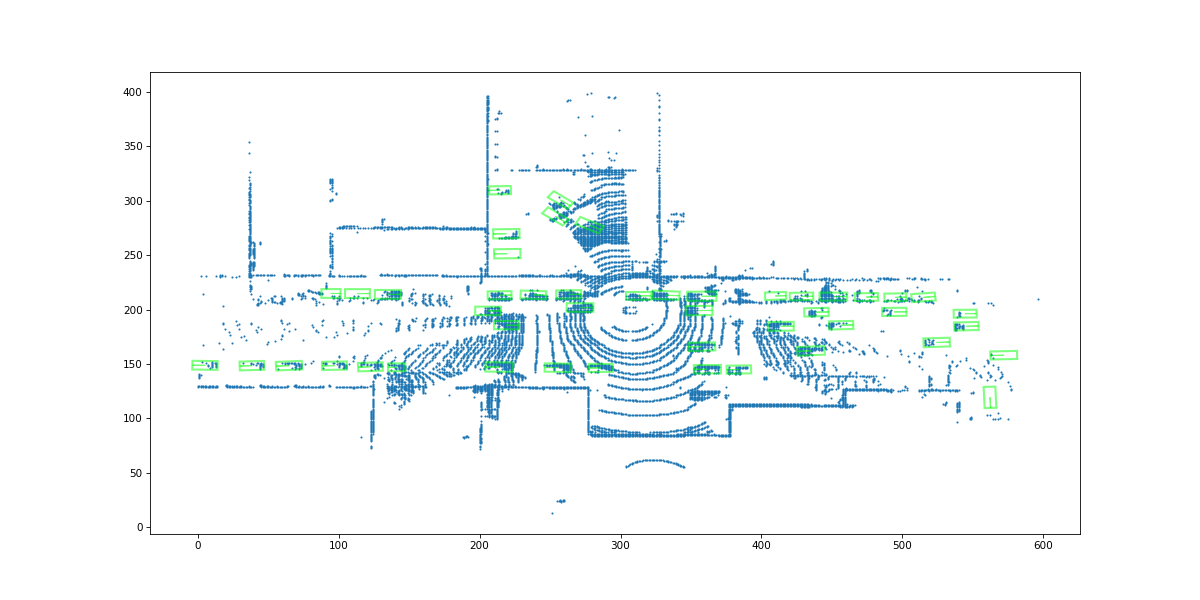
\includegraphics[width=\linewidth]{images/vox000_step0-25.png}
			\caption{step = 0.25}
		\end{subfigure}
		\vspace*{1mm}
	  
		\begin{subfigure}[t]{\textwidth}
			\centering
			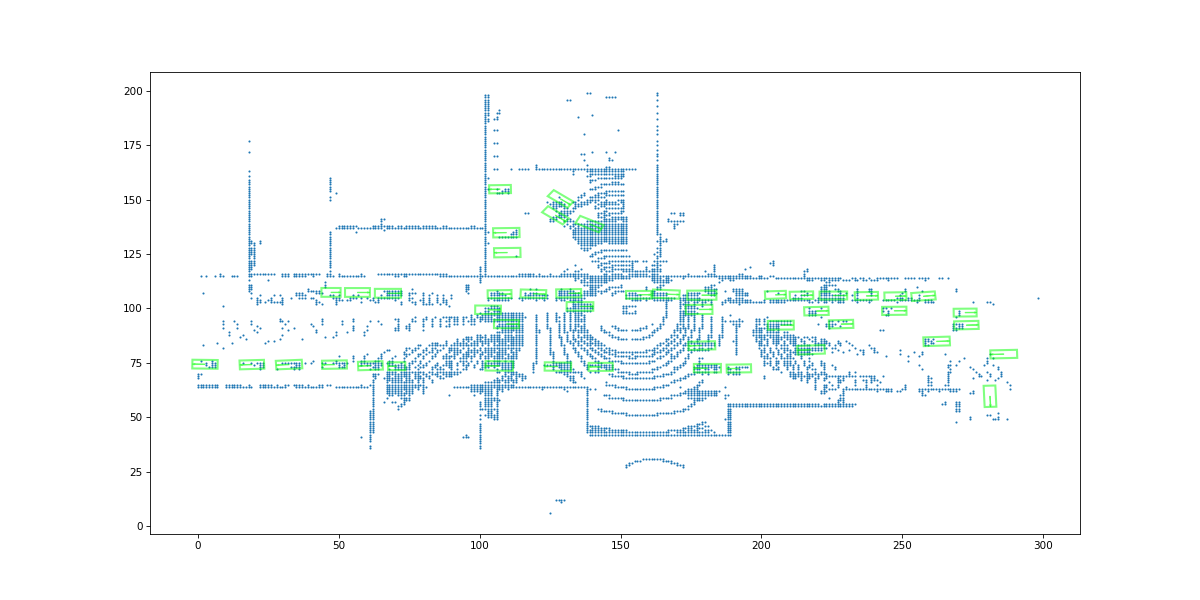
\includegraphics[width=\linewidth]{images/vox000_step0-50.png}
			\caption{step = 0.50}
		\end{subfigure}

		\caption{Voxelized LiDAR point clouds, part 1}
	\end{figure}

	\begin{figure}[h]
		\begin{subfigure}[t]{\textwidth}
			\centering
			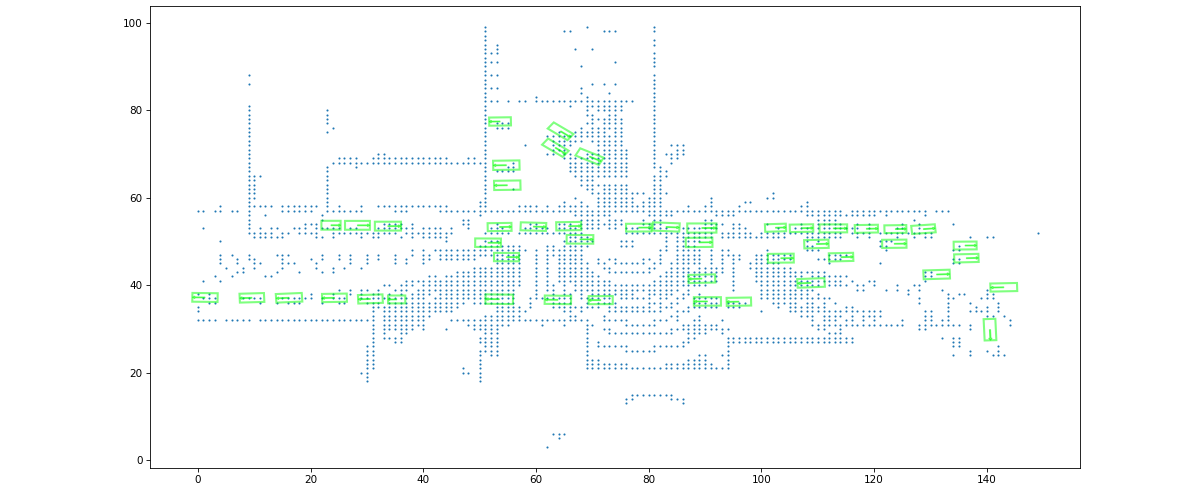
\includegraphics[width=\linewidth]{images/vox000_step1-00.png}
			\caption{step = 1.00}
		\end{subfigure}
		\vspace*{1mm}
	  
		\begin{subfigure}[t]{\textwidth}
			\centering
			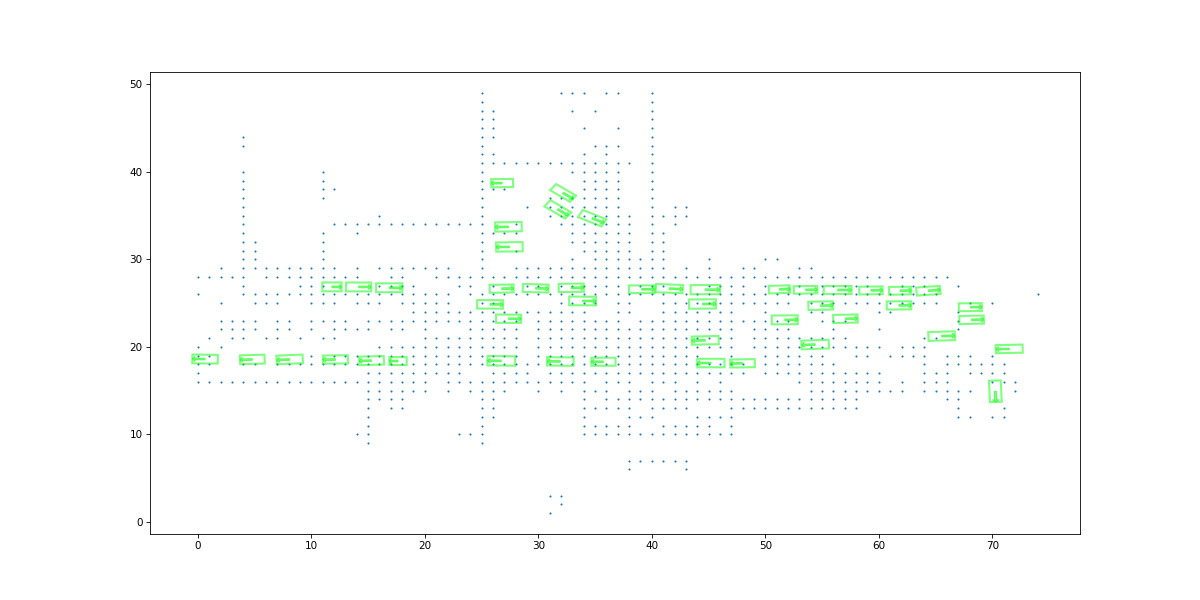
\includegraphics[width=\linewidth]{images/vox000_step2-00.png}
			\caption{step = 2.00}
		\end{subfigure}

		\caption{Voxelized LiDAR point clouds, part 2}
	\end{figure}

	From the plots above and below, we can see that the image with the highest resolution (Figure 1.a) captures much more information than the image with the lowest resolution (Figure 2.b). However, in order to have high fidelity of the voxel grid, the grid size also needs to be larger. Namely, image (Figure 1.a) has a size of 600 by 400 while image (Figure 2.b) has a size of 75 by 50; the size of the former grid is 64 times larger than the latter. 

	Therefore, we can conclude that the fidelity of the voxel grid comes at the cost of larger memory consumption (to store the larger grid). In addition, performance is also sacrificed as more captured information (voxel points) leads to more intensive computations. 

	\subsection{Model Training \& Inference}

	\textbf{Part 5:} We overfit the detector to a single frame of PandaSet using the \verb|overfit| command. The resulting detections after overfitting perfectly matches all labeled vehicles in centroids, sizes, and headings. 

	In the figure below (Figure 3), the green boxes represent the ground truth labels and the red boxes represent the detections:

	\begin{figure}[h]
		\centering
		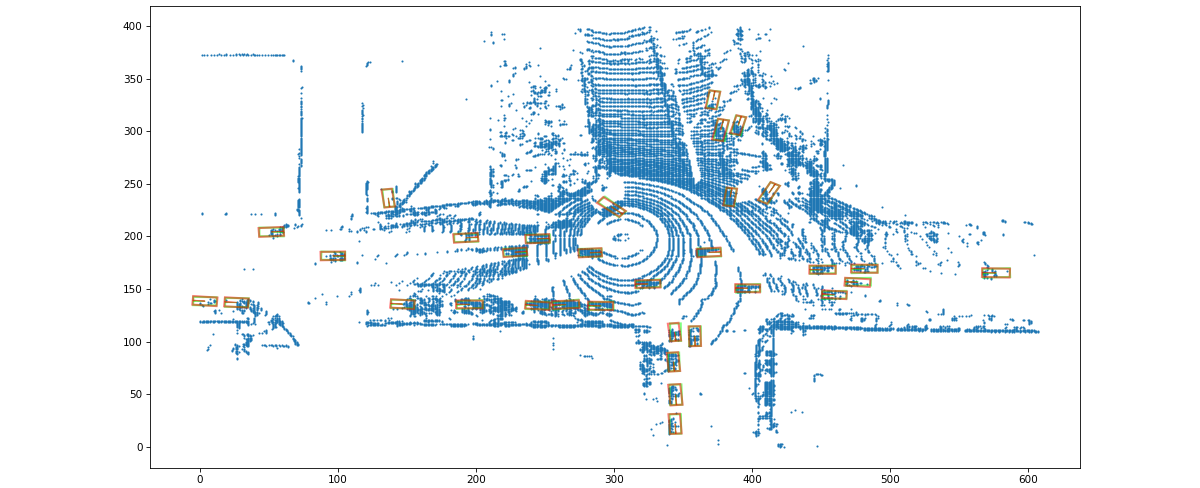
\includegraphics[width=\linewidth]{images/det_overfit.png}
		\caption{Detections after overfitting a single frame of PandaSet}
		\label{Label}
	\end{figure}

	\pagebreak
	\textbf{Part 6:} The original PandaSet dataset contains 47 sequences of LiDAR point clouds captured in intervals of 100ms. We first use 27 sequences to train the detector, then test the trained model on 12 different sequences for validation. Figure 4 below shows the detections of the model on four frames from the validation sequences.

	\begin{figure}[h]
		\begin{subfigure}[t]{0.49\textwidth}
			\centering
			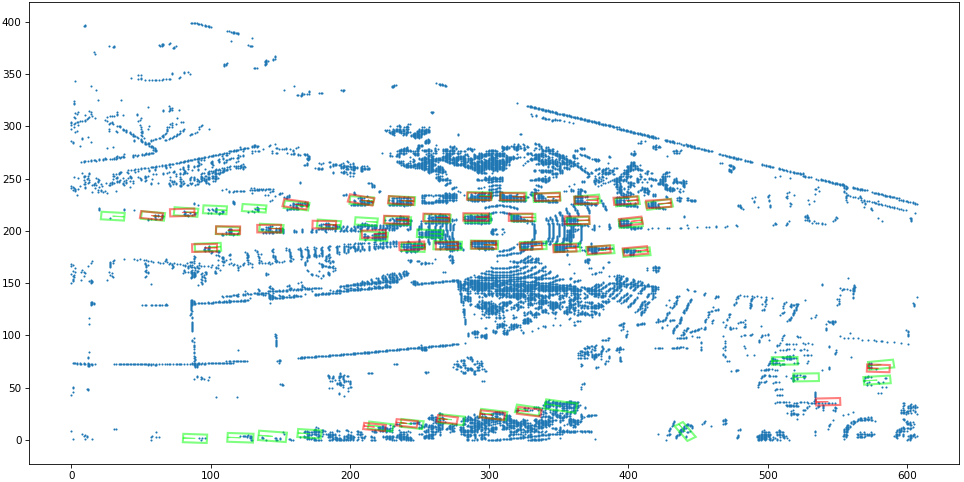
\includegraphics[width=\linewidth]{images/det_332.png}
			\caption{Detections for frame 332}
		\end{subfigure}
		\begin{subfigure}[t]{0.49\textwidth}
			\centering
			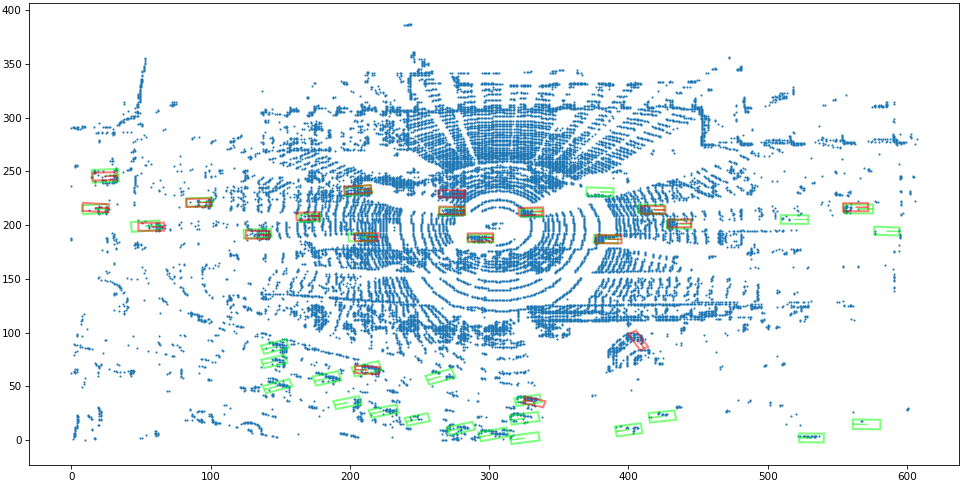
\includegraphics[width=\linewidth]{images/det_457.png}
			\caption{Detections for frame 457}
		\end{subfigure}
		\vspace*{1mm}
	  
		\begin{subfigure}[t]{0.49\textwidth}
			\centering
			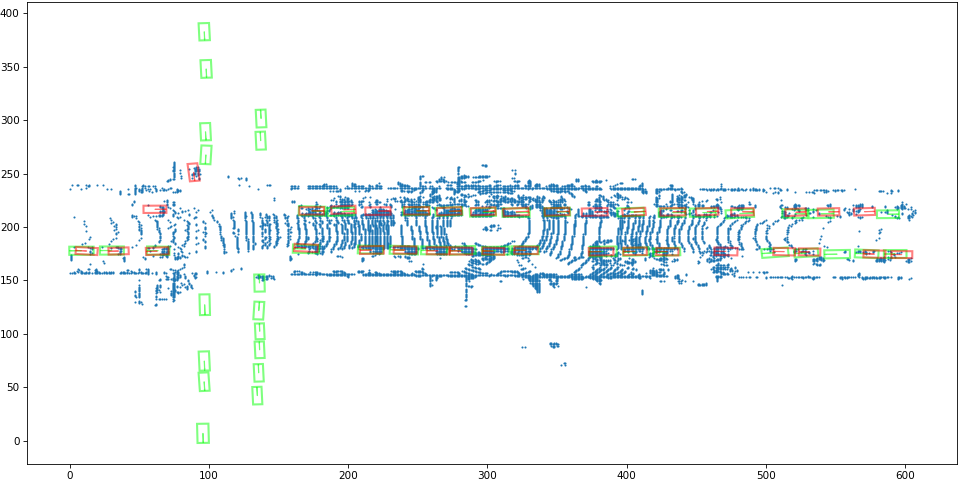
\includegraphics[width=\linewidth]{images/det_592.png}
			\caption{Detections for frame 592}
		\end{subfigure}
		\begin{subfigure}[t]{0.49\textwidth}
			\centering
			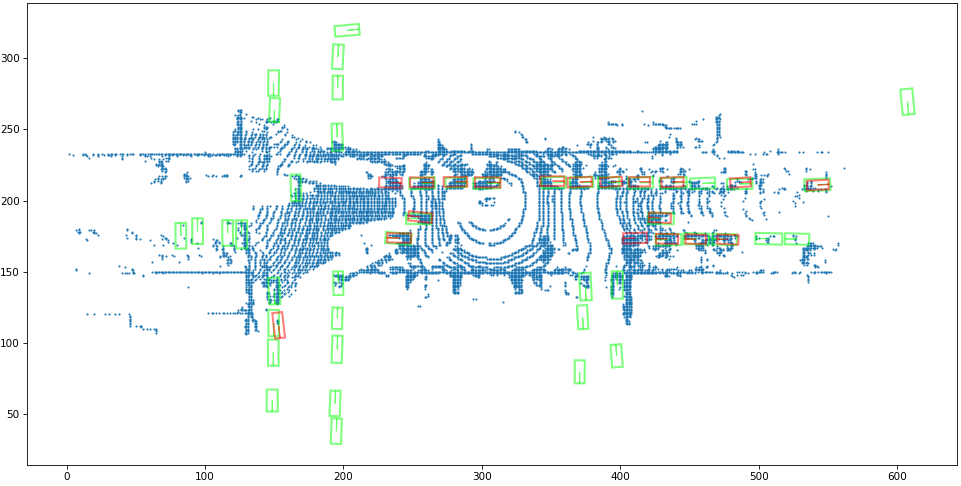
\includegraphics[width=\linewidth]{images/det_663.png}
			\caption{Detections for frame 663}
		\end{subfigure}

		\caption{Detections on frames from the validation sequences}
	\end{figure}

	From the four example frame detections above, we can see that the trained detector does a good job on detecting the centroids, sizes, and headings of the vehicles on the road, but performs poorly for vehicles off the road. This is likely due to the vehicles on the road are closer to the LiDAR sensors thus have more information captured in the LiDAR point clouds; note that some vehicles off the road do not have a single voxel in the grid. In addition, more vehicles would be detected if we adjust the activation heat threshold down, to allow the model to detect less confident vehicles. However, this would also increase the number of false positive detections. 

\end{document}
